\documentclass[10 pt, a4paper]{article}
\usepackage{amsmath}
\usepackage{tkz-euclide}
\usetkzobj{all}
\usepackage{bbding}
\usepackage{pifont}
\usepackage{wasysym}
\usepackage{amssymb}
\usepackage{tikz}
\usetikzlibrary{arrows}
\begin{document}
\title{Mathematical Finance M551 \linebreak Section 8.5  \linebreak Indiana University East}
\author{}
\date{}
\maketitle

To determine the no-arbitrage price of a call using the Black-Scholes formula, the parameters $s,t,k,r$ and $\sigma$ are needed. Of these parameters, $s,t,k, \text{ and } r$ are known. The value of $\sigma$ must be estimated. \\

In this seciton, we will investigate two techniques for estimating $\sigma$: the historical approach, and the standdard approuch. \\

Suppose $X_1,X_2,...,X_n$ are independent random variables each with the same probability distribution ( we call such random variables \textit{i.i.d.}: independent, identically distributed. \\

Suppose each $X_i$ has mean $\mu$ and variance $\sigma^2$. Then $\bar{X}$ defined by
$$\bar{X}=\frac{\sum_{i=1}^n X_i}{n}$$
is a usual estimator of the mean. In fact, $\bar{X}$ is call an 'unbiased' estimator of $\mu_0$ because $E[\bar{X}]=\mu_0$(prove this). \\

Further, the random varibale $S^2$ defined by $$S^2=\frac{\sum_{i=1}^n(x_i-\bar{x})^2}{n-1}$$ is an unbiased estimator of the variance $\sigma^2_0$, i.e. $E[S^2]=\sigma^2_0$. \\

Hence, if $C_0,C_1,...,C_n$ represent closing prices of a stock over $n+1$ days then, defining $$X_i=\log(\frac{C_i}{C_{i-1}})$$ gives as collection of $n$ \textit{i.i.d.} random varibles which, under the assumption that the daily stock prices follow a G.B.M., are normal with mean $\mu t$ and variance $t\sigma^2$. But $t=1$ ($C_i-C_{i-1})$ is one day).\\

So, the variance is given by $\sigma^2_0$, which can be estimated by $S^2$. This means $\sigma_0\approx\sqrt{S^2}$. \\

Thus, the volatility parameter can be estimated by $$\sigma_0\approx\sqrt{\frac{\sum_{i=1}^n(x_i-\bar{x}^2}{n-1})}$$\\

Now suppose we wish to estimate $\sigma$ (the volatility parameter) over an interval of time $t$ of historical data. \\

So we assume the present time is $t$ and that we have historical price data $S(y)$ for our stock, where $0\leq y\leq t$. \\

Partition the interval $[0,t]$ by fixing $n$ and letting $L=\frac tn$. \\
\begin{center}
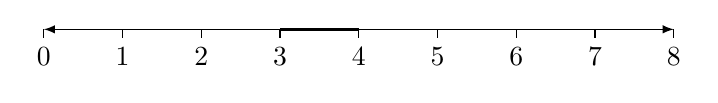
\begin{tikzpicture}
	\draw[latex-latex](0,0) --(8,0);
	\foreach \x in {0,1,2,3,4,5,6,7,8}
	\draw[shift={(\x,0)},color=black](0pt,0pt)--(0pt,-3pt)node[below]{$\x$};
	\draw[very thick](3,0)--(4,0);
\end{tikzpicture}
$$\frac tn=1$$
\end{center}
Define the random variables $X_1,X_2,...,X_n$ by\\
$$X_1=\log(\frac{S(\ell)}{S(0)})$$
$$X_2=\log(\frac{S(2\ell)}{S(\ell)})$$
$$X_3=\log(\frac{S(3\ell)}{S(2\ell)})$$
$$.$$
$$.$$
$$.$$
$$X_n=\log(\frac{S(n\ell)}{S(n-\ell)\ell})$$
Assuming that the price evolution $S(y)$ follows a G.B.M. with parameters $\mu$ and $\sigma$, it follows that the $X_i$'s are i.i.d. normal r.v's with mean $\ell \mu$ and variance $\ell\sigma^2$.\\

We will assume $t=1$ trading year, or 252 days, and that $\ell$ represents 1 day. Hence $\ell=\frac {1}{252}$. \\

Using $X_i=\log(\frac{C_i}{C_{i-1}})$ where $C_0,C_1,...,C_n$ are $n+1$ successive closing prices, we know the $X_i$'s are independent and
$$X_i\sim N(\frac{1}{252}\mu, \frac{1}{252}\sigma^2)$$ for each $i$.\\ \textit{where increments here are days as proportion of 1 year(252 days)}\\

Hence, $$\frac{1}{252}\sigma^2\approx S^2=\frac{\sum_{i=1}^n(X_i-\bar{X})^2}{n-1}$$
So that the volatiltity parameter can be approxameted by $$\sigma\approx S\sqrt{252}$$
\end{document}
